\begin{titlepage}
\begin{center}

% Upper part of the page. The '~' is needed because \\
% only works if a paragraph has started.
~\\[3cm]
\textsc{\LARGE Licence professionnelle APSIO}\\[1cm]

\textsc{\Large Projet tuteuré}\\[1.5cm]

% Title
{ \huge \bfseries Organisation collaborative du travail \\[2cm] }

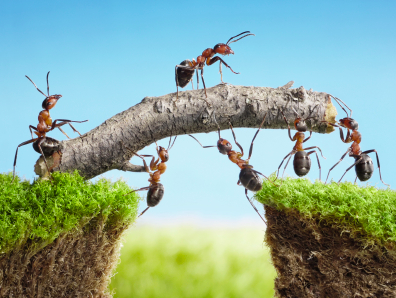
\includegraphics[width=0.7\textwidth]{img/collaborative_ants.png}~\\[1cm]

% Author and supervisor
\begin{minipage}{0.4\textwidth}
\begin{flushleft} \large
\emph{Auteur:}\\
Nathanaël \textsc{Jourdane}
\end{flushleft}
\end{minipage}
\begin{minipage}{0.4\textwidth}
\begin{flushright} \large
\emph{Tutrice :} \\
Caroline \textsc{Cambron}
\end{flushright}
\end{minipage}

\vfill

% Bottom of the page
{\large 7 octobre 2013 - \today}

\end{center}
\end{titlepage}

\newpage \strut \newpage \pagestyle{fancyplain}
